%% ------------------------------------------------------------------------- %%
\chapter{Métodos Ágeis Abertos para o OMM}
\label{cap:omm}

O objetivo do projeto QualiPSo\footnote{\url{http://www.qualipso.org}
  - Último acesso em 27/08/2010} é de aumentar a confiabilidade da
indústria e a qualidade dos sistemas livres existentes e futuros. Para
atingir esse objetivo, o projeto conta com 10 grandes áreas de
trabalho. Uma dessas áreas corresponde à confiabilidade do processo
usado no desenvolvimento de projetos livres.

Desde o início, o projeto abraçou o fato de que não poderia jamais
forçar uma forma de trabalho a comunidades livres. Por isso, a
abordagem usada para aumentar essa confiabilidade foi estabelecer uma
forma de avaliar a qualidade do processo usado por um determinado
projeto livre. Sendo assim, o projeto procurou elaborar um selo que
pudesse ser dado às comunidades que estivessem de acordo com um modelo
de processo confiável.

Porém, o contexto de projetos livre difere (como apresentado
anteriormente na Seção \ref{sec:os-def}) do contexto para ambientes
empresariais comuns. Por isso, modelos de avaliação de processos
estabelecidos na indústria não são adequados para ambientes
livres. Por isso, decidiu-se elaborar o modelo de maturidade para
software livre do Qualipso (\textit{QualiPSo Opensource Maturity
  Model} - OMM).

A seção \ref{sec:o-que-eh-omm} apresenta mais detalhes da origem do
OMM e de sua constituição. Em seguida, a seção \ref{sec:xp-em-omm}
apresenta como programação extrema pode ser mapeada para o OMM e quais
são os pontos não tratados. Por fim, a seção
\ref{sec:openagile-em-omm} apresenta uma sugestão de práticas
complementares com o objetivo de aumentar a adequação ao OMM.

\section{Origem e descrição do OMM}
\label{sec:o-que-eh-omm}

O OMM se baseia na ideia de que, na indústria, certificados de
qualidade possuam boa aceitação. Padrões como o selo
ISO9001\footnote{\url{http://www.iso.org/} - Último acesso em
  27/08/2010} ou como o Modelo de Maturidade de Capabilidade
(\textit{Capability Maturity Model} - CMM) do Instituto de Engenharia
de Software ( \textit{Software Engineering Institute} - SEI)
\footnote{\url{http://www.sei.cmu.edu/cmmi} - Último acesso em
  27/08/2010} são constituídos de documentos que descrevem uma lista
de exigências que precisam ser cumpridas nos processos das empresas
que esperaraem obter o selo.

Como projetos livres raramente beneficiam de uma infraestrutura física
ou organizacional, é muito difícil avaliar esses processos de acordo
com esses padrões da indústria. Por isso, o QualiPSo propôs trabalhar
num modelo baseado no CMM mas que pudesse ser usado não apenas para
empresas que incluem software livre em suas soluções mas também pelas
comunidades livres ao redor do mundo. Desse fato, decorre uma nota
importante sobre o OMM. O modelo todo foi pensado para que fosse
simples e fácil de usar pelos vários níveis organizacionais existentes
no ambiente de softwre livre.

A primeira fase de elaboração do OMM foi realizar um levantamento dos
chamados elementos de confiabilidade (\textit{Trusthworthy elements})
no contexto de software livre. Os elementos identificados formaram a
base do OMM para garantir que o processo avaliado não apresentasse
apenas qualidade e confiabilidade do ponto de vista comercial mas
também no contexto de comunidades livres.

Levantados esses elementos de confiabilidade, a equipe do OMM realizou
um mapeamento das áreas de qualidades avaliadas no CMM para
identificar quais elementos eram abordados e quais não eram. Os
principais elementos de confiabilidade que o CMM não aborda estão
relacionados aos problemas legais do uso de software e à reputação de
determinado projeto além do tamanho de sua comunidade.

No aspecto legal, as questões do licenciamento do código, da violação
de patentes e preservação de marcas são pontos importantíssimos para
permitir o uso de qualquer projeto livre numa organização
comercial. Na questão das contribuições, é importante tomar cuidado
com a questão dos direitos autorais para evitar problemas legais
relacionados ao licenciamento do código.  Esses dois aspectos não são
tratados ou sequer abordados no CMM porque a existência de uma
organização responsável por qualquer desenvolvimento e de regras
contratuais estabelecidas evita esses problemas.

Por outro lado, o CMM aborda alguns aspectos que são importantes para
a confiabilidade de um projeto no contexto comercial. Muitos desses
aspectos estão ligados a exigências na quantidade e detalhamento de
documentos usados para inspeção e melhoria dentro da organização que
implementa o processo. A equipe do OMM selecionou todas as práticas
sugeridas pelo CMM no que diz respeito aos aspectos técnicos e apenas
algumas no aspecto gerencial que fazem sentido no contexto livre.

Graças a esse trabalho, o OMM foi formado com um misto de elementos de
confiabilidade vindos da comunidade de software livre com práticas
estabelecidas vindas do CMM. O modelo ainda optou por adotar uma
estrutura piramidal semelhante à do CMM na qual existem três níveis de
adequação sendo que o mais básico é base para os mais avançados que
sempre exigem todas as práticas do nível inferior e mais algumas.

A Figura \ref{fig:piramide-omm} apresenta a divisão de níveis com a
lista de práticas (com nomes abreviados) que integra cada um dos
níveis do OMM. Além disso, o OMM propõe exigências diferentes de
acordo com o tipo de entidade que deseja ser avaliada para um
determinado nível. Isto é, algumas práticas são apenas recomendadas e
não obrigatórias para comunidades livres não representadas por uma
empresa. Dessa forma, quando o projeto não tem uma organização por
trás, os membros da comunidade só precisam realizar o que está no
alcance de uma comunidade para atingir um determinado nível.

% TODO Traduzir figura
\begin{figure}
  \centering
  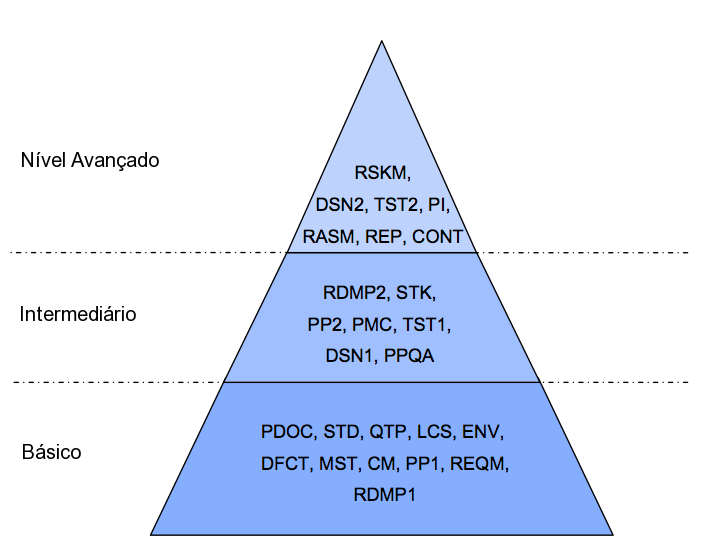
\includegraphics[scale=0.4]{omm-levels}
  \caption{Pirâmide de práticas exigidas para cada um dos níveis do
    OMM}
  \label{fig:piramide-omm}
\end{figure}

As Tabelas \ref{tab:omm-basic}, \ref{tab:omm-intermediate} e
\ref{tab:omm-advanced} mostram os elementos de confiabilidade que
precisam ser abordados para se atingir os níveis básico,
intermediário e avançados do OMM.

\begin{table}
  \begin{tabular}{|p{2cm}|p{14cm}|}
    \hline
    PDOC & Documentação do Produto (\textit{Product Documentation}) \\
    \hline
    STD & Uso de Padrões Estabelecidos e Adotados (\textit{Use of
      Established and Widespread Standards}) \\
    \hline
    QTP & Qualidade do Plano de Testes (\textit{Quality of Test Plan})
    \\
    \hline
    LCS & Licenças (\textit{Licenses}) \\
    \hline
    ENV & Ambiente Técnico (\textit{Technical Environment} -
    Ferramentas, Sistema Operacional, Linguagem de Programação,
    Ambiente de Desenvolvimento.) \\
    \hline
    DFCT & Número de Commits e Relatórios de \textit{Bugs}
    (\textit{Number of Commits and Bug Reports}) \\
    \hline
    MST & Facilidade de Manutenção e Estabilidade
    (\textit{Maintainability and Stability}) \\
    \hline
    CM & Gestão de configuração
    (\textit{Configuration Management}) \\
    \hline
    PP1 & Planejamento de Projeto Parte 1
    (\textit{Project Planning Part 1}) \\
    \hline
    REQM & Gestão de Requisitos
    (\textit{Requirements Management}) \\
    \hline
    RDMP1 & Disponibilidade de um plano
    (\textit{Availability of a Roadmap}) \\
    \hline
  \end{tabular}
  \caption{Elementos essenciais no nível básico do OMM}
  \label{tab:omm-basic}
\end{table}

\begin{table}
  \begin{tabular}{|p{2cm}|p{14cm}|}
    \hline
    RDMP2 & Desenvolvimento de um plano
    (\textit{Implementation of a Roadmap}) \\
    \hline
    STK & Relações entre interessados
    (\textit{Relationship between Stakeholders} - Usuários,
    Desenvolvedores etc) \\
    \hline
    PP2 & Planejamento de Projeto Parte 2
    (\textit{Project Planning Part 2}) \\
    \hline
    PMC & Monitoramento e Controle do Projeto
    (\textit{Project Monitoring and Control}) \\
    \hline
    TST1 & Testes Parte 1
    (\textit{Test Part 1}) \\
    \hline
    DSN1 & Projeto Parte 1
    (\textit{Design Part 1}) \\
    \hline
    PPQA & Garantia de Qualidade no Processo e no Projeto
    (\textit{Process and Project Quality Assurance}) \\
    \hline
  \end{tabular}
  \caption{Elementos essenciais no nível intermediário do OMM}
  \label{tab:omm-intermediate}
\end{table}

\begin{table}
  \begin{tabular}{|p{2cm}|p{14cm}|}
    \hline
    PI & Integração do Produto
    (\textit{Product Integration}) \\
    \hline
    RSKM & Gestão de Risco
    (\textit{Risk Management}) \\
    \hline
    TST2 & Testes Parte 2
    (\textit{Tests Part 2}) \\
    \hline
    DSN2 & Projeto Parte 2
    (\textit{Design Part 2}) \\
    \hline
    RASM & Resultados das Avaliações de Terceiros
    (\textit{Results of $3^{rd}$ Party Assessments}) \\
    \hline
    REP & Reputação
    (\textit{Reputation}) \\
    \hline
    CONT & Contribuições
    (\textit{Contributions}) \\
    \hline
  \end{tabular}
  \caption{Elementos essenciais no nível avançado do OMM}
  \label{tab:omm-advanced}
\end{table}

O texto do OMM apresenta uma abordagem Objetivo-Pergunta-Métrica (GQM
- \textit{Goal Question Metric}) no qual cada elemento possui um
conjunto de objetivos que precisam ser alcançados (ou não, dependendo
do tipo de organização sendo avaliada). As perguntas são mapeadas para
práticas recomendadas com detalhes de itens que deveriam ser
encontrados para validar que a prática é seguida.

O resto do documento de descrição do OMM apresenta recomendações para
os diferentes tipos de entidades que poderiam se interessar em obter
uma certificação OMM. Também existe uma descrição extensa de como deve
ser realizada a avaliação de uma entidade com um questionário e
informações sobre como cada prática pode ser avaliada.

A próxima seção apresenta como a Programação Extrema descrita por Kent
Beck pode ser mapeada para os elementos de confiabilidade necessários
em cada nível do OMM.

\section{Um mapeamento de Programação Extrema para o OMM}
\label{sec:xp-em-omm}

Num primeiro momento, é importante explicar porque foi escolhida a
Programação Extrema ao invés de métodos ágeis em geral. Apesar dos
Métodos Ágeis apontarem valores e princípios, não chegam a descrever
práticas ou atividades nem fluxos de trabalho. Desta forma, é
necessário optar por algum método ágil específico que faça essa
descrição mais detalhada.

Programação Extrema é um dos métodos ágeis mais antigos e mais
estudados. Graças a isso, suas várias práticas e fluxos já foram
bastante analisados o que permite mapear diversas práticas a
resultados desejados.

A próxima subseção (Seção \ref{sec:xp+omm}) apresenta
práticas da Programação Extrema que contribuem para atingir algum
objetivo do nível básico do OMM. Em seguida, a Seção \ref{sec:xp-omm}
apresenta os objetivos que ainda não foram cobertos por nenhuma
prática de Programação Extrema.

\subsection{Práticas de Programação Extrema que contribuem com o OMM
  básico}
\label{sec:xp+omm}

O OMM no nível básico se divide em 11 elementos essenciais. Essa Seção
está subdividida de acordo com os elementos cobertos por alguma prática
de Programação Extrema. Sendo assim, as próximas subseções abordarão
cada uma dos elementos essenciais e as práticas que ajudam a atingir
seu objetivo.

\subsubsection{Documentação do Produto (PDOC)}
\label{sec:+pdoc}

Uma das críticas comuns à Programação Extrema é que não se cria
nenhuma documentação sobre o sistema. Para abordar esse assunto, é
importante notar que existem dois tipos diferentes de documentação
conforme descrito no Objetivo PDOC 1 do OMM. A documentação para
desenvolvedores e a documentação para usuários.

A prática de Desenvolvimento Dirigido por Testes (TDD - \textit{Test
  Driven Development}) e sua complementação Desenvolvimento Dirigido
por Comportamento (BDD - \textit{Behavior Driven Development} são
práticas de \textit{design} mas possuem o efeito colateral de prover
diversos exemplos de uso do código criado. A ideia do BDD separa o
teste no sentido de verificação de entrada e saída do comportamento
desejado com aquele teste graças ao uso consciente de nomes de testes
que descrevam o comportamento desejado.

Diversas ferramentas de BDD (como
JBehave\footnote{\url{http://jbehave.org/} - Último acesso
  29/09/2010}, RSpec\footnote{\url{http://rspec.info/} - Último acesso
  29/09/2010} e
DocTest\footnote{\url{http://docs.python.org/library/doctest.html} -
  Último acesso 29/09/2010}) possuem relatórios de execução que
produzem saídas em formato de documentos. Esses relatórios apresentam
descrições de como os módulos do sistema funcionam de acordo com os
testes que foram escritos para eles. Dessa forma, não somente o
sistema ganha uma documentação estensa, como também existe a garantia
que esta documentação será mantida atualizada ou pelo menos informará
que o sistema mudou com relação a ela.

Dessa forma, a prática de TDD/BDD ajuda a atingir o objetivo descrito
pela Prática PDOC 1.1 que exige a criação de uma documentação para
desenvolvedores. Caso o relatório de documentação seja gerado
automaticamente na construção do projeto, essa prática também ajuda a
atingir o objetivo PDOC 3 que pede que a documentação seja melhorada
com o produto.

Ainda com relação à área de Documentação (PDOC), a prática PDOC 1.3
que pede pela criação de documentações genéricas do produto pode ser
cumprida com a realização do planejamento da iteração e a coleta de
seus resultados em uma ferramenta online (como
XPlanner\footnote{\url{http://xplanner.org/} - Último acesso em
  29/09/2010},
Mingle\footnote{\url{http://studios.thoughtworks.com/mingle-agile-project-management}
  - Último acesso em 29/09/2010},
Calopsita\footnote{\url{http://calopsitaproject.com/} - Último acesso
  em 29/09/2010} etc). Dessa forma, a documentação do que foi planejado em
cada fase do produto assim como o andamento até o momento naquela fase
é atualizado automaticamente conforme os desenvolvedores completam
suas tarefas.

\subsubsection{Uso de Padrões Estabelecidos e Adotados (STD)}
\label{sec:+std}

Apesar de Kent Beck não mencionar nenhuma prática com relação às
ferramentas usadas no desenvolvimento dos projetos, as práticas de
Código Compartilhado e de \textit{Design} Simples encorajam o
desenvolvimento de aplicações para as quais é fácil um desenvolvedor
participar ativamente do desenvolvimento de um projeto em pouco
tempo. Sendo assim, o uso de padrões abertos amplamente difundidos e
utilizados reduz a necessidade de treinamento.

Portanto, pode-se argumentar que a adesão a padrões abertos no produto
é uma prática que apoia as práticas de Código Compartilhado e
\textit{Design} Simples e, ao mesmo tempo, é apoiada por elas.

Além disso, a adoção de Programação Extrema é compatível com o
Objetivo STD 2 - Adotar processos de desenvolvimento padrões - já que
Programação Extrema é um processo aberto e livre.

\subsubsection{Qualidade do Processo de Testes (QTP)}
\label{sec:+qtp}

Novamente, a prática de TDD/BDD e suas variações como Desenvolvimento
Dirigido por Testes de Aceitação (ATDD - \textit{Acceptance Test
  Driven Development}), apesar de serem técnicas essencialmente ligadas
ao \textit{design} do projeto, tem como efeito colateral a criação e
manutenção de testes em vários níveis (Testes de unidade, de integração
e de sistema ou integração de sistema dependendo do objetivo do
projeto). Dessa forma, o uso conjunto de TDD, BDD e ATDD permite
atingir o Objetivo QTP 1 (Prover um plano de alta qualidade de testes)
já que o plano é a descrição e implementação dos testes logo antes da
realização da funcionalidade e decorre diretamente do plano de desenvolvimento.

Também cobre-se o Objetivo QTP 2 (Implementar o gerir o processo de
testes) com essas práticas de XP já que o desenvolvimento e execução
dos testes é garantida antes, durante e após a implementação das
funcionalidades associadas. A prática de Integração
Contínua contribui para o Objetivo QTP 2 ao garantir que os testes são
realizados frequentemente a cada modificação da base de código
garantindo \textit{Feedback} imediato do trabalho necessário.

TDD/BDD e ATDD também garantirão que o Objetivo QTP 3 (Melhorar o
processo de testes) será atingido já que forçam o desenvolvedor a
incluir um teste antes de realizar qualquer mudança no código do
sistema. Dessa forma, correções de erros, inclusões de funcionalidades
ou melhorias de desempenho são capturadas em testes automatizados e
garantem a adequação do futuro do projeto a essas decisões.

\subsubsection{Ambiente (ENV)}
\label{sec:+env}

As práticas de Código Compartilhado, Repositório Único de Código e
Integração Contínua exigem uma organização do projeto de forma a
facilitar ao máximo a reprodução do ambiente de desenvolvimento e de
produção.

Desta forma, o repositório único de código deveria conter todos os
arquivos necessários para construir e rodar os testes automatizados do
sistema. Sendo assim, tratam-se vários pontos apontados pelo Objetivo
ENV 1 (Planejar o desenvolvimento de recursos e infra-estrutura) já
que basta saber qual o repositório único de código para conseguir
montar um ambiente de contribuição ao projeto.

A prática de Código Compartilhado exige uma padronização no estilo de
escrita de código e de teste que deve ser compartilhado por
todos. Sendo assim, os arquivos descrevendo essas padronizações devem
estar sob controle de versão no repositório único de código de forma a
serem obtidos por qualquer contribuidor.

Por fim, a prática de Integração Contínua exige um sistema automático
para obtenção do código, instalação do mesmo num ambiente limpo e
execução dos testes automatizados do projeto. Porém, para que seja possível
montar esse tipo de ambiente automaticamente, é necessário que a
descrição e configuração do ambiente de produção esteja incluída nessa
ferramenta de Integração Contínua servindo tanto de exemplo quanto de
documentação.

\subsubsection{Número de \textit{commits} e relatório de defeitos
  (DFCT)}
\label{sec:+dfct}

A prática de Repositório Único de Código exige o uso de uma ferramenta
de controle de versão. Essa ferramenta permite manter o histórico de
qualquer alteração realizada nos arquivos sob controle de
versão. Dessa forma, é muito fácil obter qual o número de
\textit{commits} realizados e o que cada \textit{commit} procurava
resolver.

Com relação ao relatório de defeitos, a prática de Histórias exige que
qualquer mudança que precisa ser realizada no projeto passe pela
escrita de uma História. Sendo assim, qualquer relatório de defeito
pode ser apresentado na forma de uma tarefa que precisa ser realizada
e descrita como uma História. Dessa forma, relatar um defeito é
equivalente a escrever uma História e inserí-la no conjunto de
histórias do projeto.

O uso de ferramentas para gestão de projeto online (como as citadas na
Seção \ref{sec:+pdoc}) permite que o cadastro dessas Histórias seja
realizado de forma simples e direta. A forma de contribuir com
alterações de código ou documentação relacionados a uma determinada
História varia um pouco de acordo com o sistema de controle de versões
usado. Em ferramentas para controle de versão distribuídas, a melhor
forma de contribuir com sugestões de mudanças é apenas incluir um
\textit{link} para o controle de versão com as mudanças. Numa
ferramenta de controle de versão tradicional, o melhor seria gerar um
arquivo com as diferenças entre o código original e o código
alterado. De qualquer forma, incluir essas sugestões é tão simples
quanto anexar um arquivo ou incluir um \textit{link}.

Dessa forma, cobre-se o Objetivo DFCT 1 ao prover uma forma
padronizada e simples de contribuir com o projeto. O uso de uma
ferramenta de controle de versão atualizada (como pede a prática
Repositório Único de Código) também ajuda a atingir o Objetivo DFCT 2
que exige uma gestão das contribuições, \textit{commits} e relatórios
de erros.

\subsubsection{Manutenabilidade e Estabilidade (MST)}
\label{sec:+mst}

As práticas de Refatoração e Programação em Pares são essenciais em XP
para reduzir o número de defeitos inseridos no código mas também para
garantir que o código da aplicação permanece legível e mais simples de
manter. Um dos estudos mais reconhecidos sobre Programação em Pares
\cite{Williams2000} mostra que o uso de Programação em Pares reduz a
quantidade de defeitos, melhora a qualidade do \textit{design} e
distribui conhecimento técnico. Já a Refatoração \cite{Refac01} é uma
prática cujo objetivo é melhor a manutenabilidade de um determinado
código sem alterar sua funcionalidade.

Essas duas práticas aliadas ajudam a cumprir o Objetivo MST 1 que
requer um planejamento para qualidade do produto em termos de
requisitos não-funcionais. Adicionando a prática de Código e Teste é
possível garantir também que o sistema se comporte como esperado em
diversos ambientes (\textit{hardware} e software).

Já a prática de Retrospectiva aliada com a prática de Análise de Causa
Inicial irão permitir atingir o Objetivo MST 2 que procura melhorar a
qualidade do processo do projeto. A ideia da prática de Retrospectiva
\cite{Derby2006} é usar técnicas de identificação de problemas ou
pontos de melhoria e coleta de sugestões de mudanças para realizar
essas melhoras. Já a Análise de Causa Inicial permite resolver não
apenas os problemas superficiais mas também os problemas que são
fontes de problemas superficiais.

Por fim, a prática de Integração Contínua aliada com a de TDD/BDD vai
permitir atingir o Objetivo MST 3 que pede para gerenciar o processo
de manutenabilidade. Essa gestão se dará com os resultados da
construção e execução dos testes realizados a cada mudança no
Repositório Único de Código. Esses resultados apresentam o
\textit{commit} exato que retirou uma determinada funcionalidade ou
interface de programação.

\subsubsection{Gestão de Configuração (CM)}
\label{sec:+cm}

A prática de Código Compartilhado pede que qualquer desenvolvedor do
sistema tenha o direito e a possibilidade de alterar qualquer trecho
de código independente de quem foi o autor desse trecho ou quando ele
foi criado. Para que isso seja possível, o projeto deve estabelecer
padrões de estrutura de arquivos, formatação usada além de estilo de
nomenclatura e outros itens que permitem uma integridade conceitual
para o código do projeto.

Esses padrões iniciais estabelecem uma configuração padrão para
qualquer desenvolvedor e podem ser integrados ao sistema de controle
de versão do Repositório Único de Código para garantir a gestão e
distribuição desses arquivos de forma consistente. Esses arquivos
contribuem com o Objetivo CM 1 que pede o estabelecimento de linhas de
base para o desenvolvimento do produto.

As práticas de História e de Ciclos (Semanais e de Estação) permitem
também manter um acompanhamento de quando as Histórias são criadas e
quando elas são planejadas para serem desenvolvidas. Manter o
histórico dessas Histórias e Ciclos permite atingir o Objetivo CM 2 de
acompanhar e controlar mudanças às configurações do projeto.

\subsubsection{Planejamento de Projeto 1 (PP1)}
\label{sec:+pp1}

A prática de Jogo do Planejamento pede que a equipe de desenvolvimento
trabalhe com o cliente ou usuário do sistema e decide qual será o
trabalho a ser realizado no próximo Ciclo Semanal. Durante essa
reunião, o usuário define quais são as Histórias que precisam ser
realizadas com maior prioridade. Seguindo essa ordem de prioridades,
os desenvolvedores pensam sobre a dificuldade para realizar aquela
História considerando suas experiências passadas e estimando
comparativamente. Dessa forma, estabelecem-se estimativas para as
Histórias mais importantes até que o cliente consiga escolher um
conjunto de histórias que preencha o Ciclo Semanal.

Dessa forma, ao final de um Jogo do Planejamento, o projeto tem uma
estimativa para o escopo a ser realizado durante aquele ciclo, o
esforço/custo e duração para realização dessas tarefas e uma
estimativa crua de tarefas futuras. Essas estimativas ajudam a atingir
o Objetivo PP1 1 que pede o estabelecimento de estimativas.

O Jogo do Planejamento ainda diz que as Histórias que forem
consideradas de maior valor de negócio e de maior risco são as que tem
maior prioridade no desenvolvimento. Dessa forma, a equipe precisa
informar junto com a estimativa da história qual o risco técnico associado com
aquela história e o cliente deve saber o risco de negócios
relacionado. Com essas duas informações, o plano de desenvolvimento do
projeto decorre da regra de sempre trabalhar nas histórias de maior
risco e maior valor existente atualmente. Dessa forma, caso o projeto
encontre um grande problema, isso acontecerá cedo no processo.

Esse planejamento de desenvolvimento do projeto é o Objetivo PP1 2 que
corresponde ao Ciclo de Estação do Produto.

\subsubsection{Gestão de Requisitos (REQM)}
\label{sec:+reqm}

A prática de Histórias consiste em coletar de forma concisa e curta uma
necessidade do ponto de vista de negócio para o projeto. Essa história
é inicialmente apresentada como uma descrição muito curta e muito
simples mas é associada com a pessoa que a requisitou. Dessa forma,
caso essa história seja escolhida para o Ciclo Semanal, os
desenvolvedores tem a possibilidade de obter mais informações sobre o
trabalho a ser realizado. As reuniões do Jogo do Planejamento permitem
revisar e atualizar essas histórias de forma a garantir a gestão com
relação às mudanças nos requisitos descritos pela história. Com isso,
é possível cumprir o Objetivo REQM 1 que pede uma gestão de
requisitos.

\subsection{Resumo}
\label{sec:resumo-omm}

Em resumo, as seguintes práticas de Programação Extrema foram
associadas aos seguintes elementos essenciais do OMM:

%TODO Trocar por uma tabela com checks (linhas são práticas e colunas
%são elementos essenciais do OMM)
\begin{enumerate}
\item Código Compartilhado

  Relacionada aos elementos essenciais: STD, ENV, MST e CM.
\item \textit{Design} Simples

  Relacionada aos elementos essenciais: STD.
\item Repositório Único de Código

  Relacionada aos elementos essenciais: ENV, DFCT, MST e CM.
\item Integração Contínua

  Relacionada aos elementos essenciais: QTP, ENV, CM e REQM.
\item Programação em Pares

  Relacionada aos elementos essenciais: STD e MST.
\item Código e Teste

  Relacionada aos elementos essenciais: QTP e MST.
\item TDD

  Relacionada aos elementos essenciais: PDOC, QTP, DFCT e MST.
\item Refatoração

  Relacionada aos elementos essenciais: ENV e MST.
\item Ciclo Semanal

  Relacionada aos elementos essenciais: PP1 e CM.
\item Ciclo de Estação

  Relacionada aos elementos essenciais: PP1, CM e REQM.
\item Retrospectiva

  Relacionada aos elementos essenciais: MST.
\item Análise de Causa Inicial

  Relacionada aos elementos essenciais: MST.
\item Histórias

  Relacionada aos elementos essenciais: PP1, DFCT, CM e REQM.
\item Jogo do Planejamento

  Relacionada aos elementos essenciais: PP1 e REQM.
\end{enumerate}

A Seção a seguir (Seção \ref{sec:xp-omm}) apresenta os elementos
essenciais e partes de objetivos que não foram atingidos com as
práticas de XP listadas até agora.

\subsection{Elementos essenciais não cobertos pela Programação
  Extrema}
\label{sec:xp-omm}

Os principais elementos que não foram cobertos pelas práticas de XP
são:

\begin{enumerate}
\item PDOC - Objetivo 1.2

  - Criar uma documentação para usuários

\item PDOC - Objetivo 2

  - Criar um a documentação pro produto

\item STD - Objetivo 3

  - Garantir independência estratégica do projeto

\item LCS

  Toda a parte de Licenças

\item ENV - Objetivo 3

  Melhorar o uso de ferramentas livres

\item CM - Objetivo 3

  Estabelecer Integridade

\item RDMP1 - Objetivo 1

  Planejar o plano do produto
\end{enumerate}

Com relação ao Item 1, XP defende que a documentação para o usuário
deve ser incluída como uma História como qualquer outra. Nesse ponto,
ela pode ser priorizada e incluída no Ciclo Semanal como qualquer
outra funcionalidade. Sendo assim, o processo não garante que a
documentação para o usuário será desenvolvida mas garante que, se ela
for importante, ela será realizada.

Nesse ponto, a melhor opção pode ser incluir a escrita de documentação
para usuário junto com a história da funcionalidade. Dessa forma,
garante-se que a História não é aprovada (ou terminada) caso não
exista essa documentação.

O item 2 cai numa situação similar. Implementar uma documentação
embutida no produto é uma funcionalidade como outra que deveria ser
priorizada e incluída no Ciclo Semanal como outras. O ponto a destacar
é apenas que, uma vez que o sistema estiver desenvolvido, ele deveria
ser realizado de tal forma que a documentação para o usuário
refletisse na documentação para o produto em si.

O item 3 é um pouco mais complicado de tratar já que envolve analisar
cada uma dos padrões para avaliar a chance dele causar uma dependência
futura. Para conseguir atingir esse objetivo, é necessário incluir
alguma prática de análise de risco para os componentes usados na
implementação de cada História.

O item 4 é similar mas em geral terá um peso mais significativo apenas
no início do projeto. Sendo assim, talvez seja importante dedicar um
ciclo semanal de preparação e análise do projeto para averiguar as
possibilidades no quesito de licenças que o projeto aceita.

O item 5 envolve pesquisa em busca de componentes abertos para
substituir componentes proprietários. Dessa forma, o processo
precisaria incluir inspeções recorrentes dos componentes e ferramentas
usadas em busca de alternativas livres.

O item 6 é provavelmente um dos objetivos mais difíceis de
atingir. Integridade Conceitual é um requisito que já é difícil
conseguir quando uma única pessoa realiza todo o trabalho. No contexto
de uma equipe com contribuições externas (como o cenário de software
livre), transmitir o conceito do projeto é bem complicado. Nesse caso,
a sugestão seria de incluir pequenas conversas entre os
usuários/clientes e desenvolvedores gravadas (aúdio e vídeo)
disponíveis na página \textit{Internet} do projeto.

O item 7 pode ser obtido ao estabelecer uma cadência para os ciclos de
estação e realizar Jogos do Planejamento em vários níveis ao final de
cada estação. XP defende que esse tipo de planejamento a longo prazo
deveria ser realizado apenas num nível bem geral para permitir
mudanças que ocorrerão inevitavelmente.

Sendo assim, a Seção \ref{sec:openagile-em-omm} apresenta uma variação
de XP que cobre os níveis básicos do OMM com as sugestões anteriores.

\section{Um proposta ágil compatível com o OMM}
\label{sec:openagile-em-omm}

